\documentclass[unicode, 8pt]{beamer}
\usetheme{Madrid}
\usecolortheme{seahorse}     %цветовая схема
\useinnertheme{circles}   %внутренняя тема
\usefonttheme{serif}    %шрифты

\usepackage[utf8]{inputenc}
\usepackage[T2A]{fontenc}
\usepackage[russian]{babel}
\usepackage[listings,theorems]{tcolorbox}
\usepackage{caption}
\usepackage[labelsep=period]{caption}
\setbeamertemplate{caption}[numbered]
\graphicspath{{../pic}}

\definecolor{shBlue}{HTML}{d6d6f0}
\definecolor{lightGray}{HTML}{F5F5F5}
\definecolor{spGreen}{HTML}{93DDC2}
\definecolor{spBlue}{HTML}{007AFF}
\definecolor{mainBackground}{HTML}{F9FEFC}

\makeatletter
\newcommand*{\rom}[1]{\expandafter\@slowromancap\romannumeral #1@}
\makeatother

\newcommand{\picref}[1]{рис. \ref{#1}}
\newcommand{\half}{\frac{1}{2}}
\newcommand{\dhalf}{\dfrac{1}{2}}
\newcommand*{\Scale}[2][4]{\scalebox{#1}{$#2$}}


\setbeamercolor{block title}{bg=shBlue!70,fg=black}
\setbeamercolor{block body}{bg=lightGray!50,fg=black}
% \setbeamercolor{frametitle}{fg=selected,bg=spGreen}
% \setbeamercolor{background canvas}{bg=mainBackground}
\setbeamertemplate{blocks}[rounded][shadow=false]

\title[Курсовая работа]{Кусочно-параболический метод на локальном шаблоне для решения гиперболических уравнений в частных производных}
\author[Токарев А.\,И.]{Выполнил: Токарев~А.\,И.\\[1ex]  {Научный руководитель: Лукин~В.\,В.}}
\institute[]{МГТУ им. Н.Э. Баумана}
\date{\today}

\begin{document}

    \begin{frame}
        \titlepage
    \end{frame}

    \begin{frame}
        \frametitle{Содержание}
        \tableofcontents
    \end{frame}

    \section{Постановка задачи}

    \begin{frame}
        \frametitle{Постановка задачи}
        \begin{block}{Аппроксимирующая парабола внутри разностной ячейки}
            Имея значения в узлах $x_i,\, i = 0 \ldots N$, доопределяем значения в половинных узлах, то есть исходная сетка $\Omega_h = \{ x_i,\, i = 0 \ldots N \}$ преобразуется в набор отрезков $\bigl[ x_{i-\half}, x_{i+\half} \bigr]$ с определенными в них параболами:
            \begin{equation}
                \label{parabolic_eq}
                \begin{split}
                    &y(x) = y_i^L + \xi(\Delta y_i + y_i^{(6)}(1 - \xi)), \quad \xi = (x - x_{i-\half})h^{-1}, \quad  \Delta y_i = y_i^R-y_i^L, 
                    \\
                   &y_i^{(6)} = 6\Bigl[ y_i - \half(y_i^R + y_i^L)\Bigr], \quad x \in [x_{i-\half}, x_{i + \half}]. 
                \end{split}
            \end{equation}
        \end{block}

        \begin{figure}[h]
            \centering
            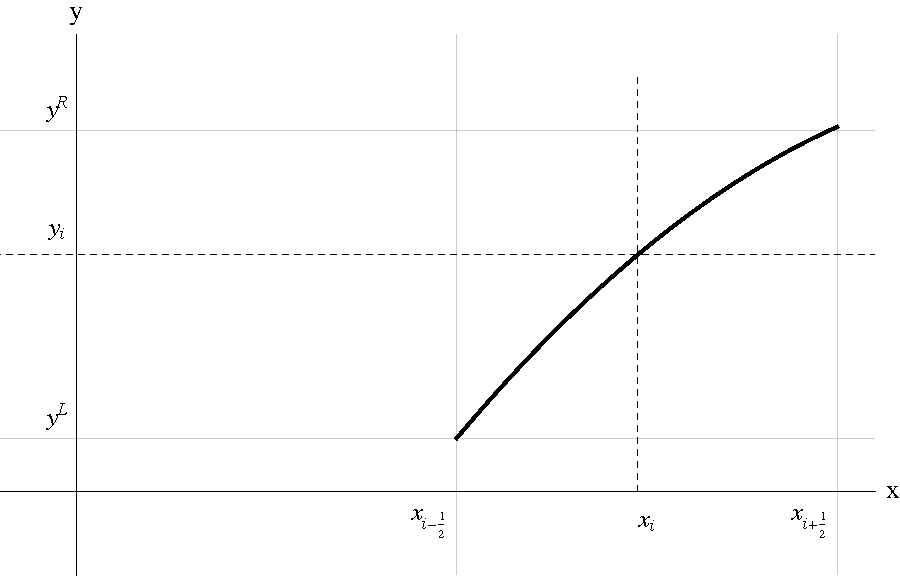
\includegraphics[width=0.47\textwidth]{ppm_visual.pdf}
            \caption{Парабола внутри разностной ячейки}
            \label{fig:ppm_visual}
        \end{figure}
    \end{frame}

    \begin{frame}{Постановка задачи}
        Для выражение \eqref{parabolic_eq} выполняется соотношение:
            \begin{equation}
                \label{average}
                \Scale[0.9] {
                    y(x_i) = \dfrac{1}{h} \displaystyle \int\limits_{x_{i-\half}}^{x_{i+\half}} y(\chi) d\chi,
                }
            \end{equation}
            \noindent то есть значения в узлах сетки $\Omega_h$ являются средними значениями (\picref{average}).

        \begin{block}{Среднее значение на отрезке}
            После определения парабол можно считать средние значения на отрезках $ [x_{i+\half}-\alpha, x_{i+\half}] $ и $ [x_{i+\half}, x_{i+\half}+\alpha]\colon $
            \begin{equation}
                \label{average_positive}
                \Scale[0.9] {
                    \overline y_{i+\half}^L(\alpha) = \dfrac{1}{\alpha} \displaystyle \int\limits_{x_{i+\half}-\alpha}^{x_{i+\half}} y(x) dx = y_i^R - \dfrac{\alpha}{2h}\Bigl[ \Delta y_i - \Bigl( 1 - \dfrac{2 \alpha}{3h} \Bigr)y_i^{(6)} \Bigr],
                }
            \end{equation}
            \begin{equation}
                \label{average_negative}
                \Scale[0.9] {
                    \overline y_{i+\half}^R = \dfrac{1}{\alpha} \displaystyle \int\limits_{x_{i+\half}}^{x_{i+\half}+\alpha} y(x) dx = y_{i+1}^L  + \dfrac{\alpha}{2h} \Bigl[\Delta y_{i+1} + \Bigl( 1 - \dfrac{2\alpha}{3h} \Bigr) y_{i+1}^{(6)} \Bigr].
                }
            \end{equation}
        \end{block}
    \end{frame}

    \section{Алгоритм}
    \begin{frame}{Алгоритм}
        \begin{block}{Граничные значения в кусочно-параболическом методе -- PPM}
            \[
                y_i^R = y_{i+1}^L = y_{i+\half} = \dhalf(y_i + y_{i+1}) - \dfrac{1}{6}(\delta y_{i+1} - \delta y_i), \quad \delta y_i = \dhalf(y_{i+1} + y_{i-1}).
            \]
            Для того, чтобы обеспечить монотонность решения, $\delta y_i$ заменяется на:
            \[
                \Scale[0.95] {
                    \delta_m y_i = 
                    \begin{cases}
                        \min(|\delta y_i|,\, 2|y_i - y_{i-1}|,\, 2|y_{i+1} - y_i|)\cdot sign(\delta y_i), & (y_{i+1} - y_i)(y_i - y_{i-1}) > 0, \\
                        0, \quad (y_{i+1} - y_i)(y_i - y_{i-1}) \leq 0.
                    \end{cases}   
                } 
            \]
        \end{block}

        \begin{block}{Модификация метода. Кусочно-параболический метод на локальном шаблоне -- PPML}
            В качестве альтернативы предлагает перенос граничных узлов по характеристикам. \\[0.5em] Пусть $ \frac{dx}{dt} = a $.
            \begin{itemize}
                \item Если $ a > 0 $, то получаем:
                \[
                    \Scale[0.95] {
                        y_{i+\half}(t_{j+1}) = y_i^R(t_{j+1}) = y_i^L(t_j) + \xi(\Delta y_i(t_j) + y_i^{(6)}(t_j)(1-\xi)), \quad \xi = 1 -  \dfrac{a \tau}{h}.
                    }
                \]        
                \item При $ a < 0 $:
                \[
                    \Scale[0.95] {
                        y_{i+\half}(t_{j+1}) = y_i^R(t_{j+1}) = y_{i+1}^L(t_j) + \xi(\Delta y_{i+1}(t_j) + y_{i+1}^{(6)}(t_j)(1-\xi)), \quad \xi = -\dfrac{a \tau}{h}.
                    }
                \]
            \end{itemize}
        \end{block}
    \end{frame}

    \begin{frame}{Алгоритм}
        \begin{figure}[h]
            \centering
            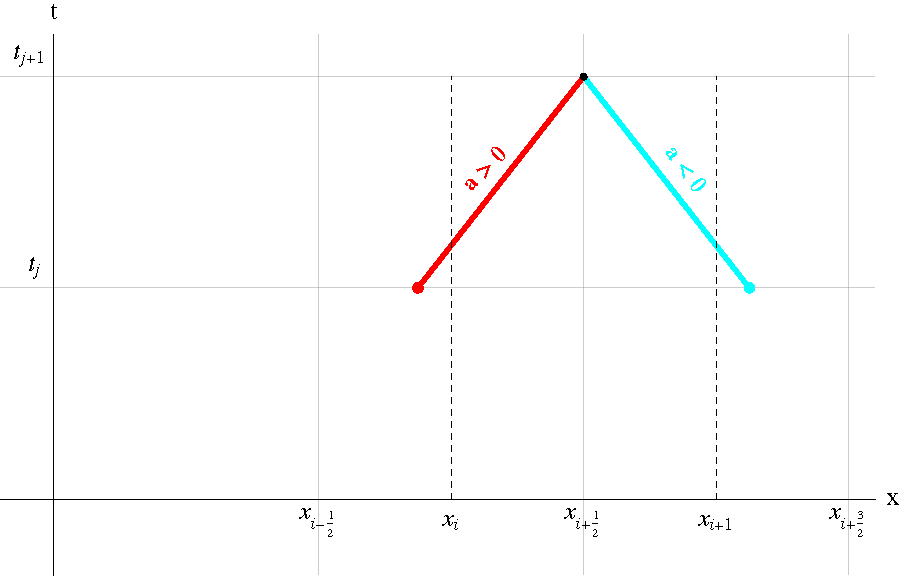
\includegraphics[width=0.4\textwidth]{ppml_visual.pdf}
            \caption{Перенос значений на границах вдоль характеристик в методе PPML}
            \label{fig:ppml_visual}
        \end{figure}
        \begin{block}{Избавление от локальных экстремумов}
            \begin{itemize}
                \item $ y_i $ является локальным экстремумом, тогда:
                \[
                    y_i^L = y_i^R = y_i, \quad (y_{i+1} - y_i)(y_i - y_{i-1}) \leq 0;
                \]       
                \item $ y_i $ лежит слишком близко к границе:
                \[
                    \begin{split}
                        y_i^L = 3y_i -2y_i^R, &\quad \Delta y_i \cdot y_i^{(6)} > (\Delta y_i)^2, \\
                        y_i^R = 3y_i -2y_i^L, &\quad \Delta y_i \cdot y_i^{(6)} < -(\Delta y_i)^2.
                    \end{split}  
                \]
            \end{itemize}
        \end{block}
    \end{frame}

    \section{Одномерное уравнение переноса}
    \begin{frame}{Одномерное уравнение переноса}
       \begin{block}{Вид уравнения и характеристики}
        \begin{equation}
            \label{convection-diffusion}
            \dfrac{\partial y}{\partial t} + a \dfrac{\partial y}{\partial x} = 0 \,\, \Rightarrow \,\, \dfrac{dx}{dt} = a \,\, \Rightarrow \,\, x = a t + b.
        \end{equation}
       \end{block}

       \begin{block}{Интегро-интерполяционный метод}
            \[
                \int \limits_{x_{i-\half}}^{x_{i+\half}} \int \limits_{t_j}^{t_{j+1}} \dfrac{ \partial y(x, t) }{ \partial t } \, dt \, dx \,\, + \int \limits_{t_j}^{t_{j+1}} \int \limits_{x_{i-\half}}^{x_{i+\half}} a \dfrac{ \partial y(x,t) }{ \partial x } \, dx \, dt \,\, = \int \limits_{x_{i-\half}}^{x_{i+\half}} \int \limits_{t_j}^{t_{j+1}} 0 \, dt \, dx \, \, = 0.
            \]
            Рассмотрим интегралы по отдельности: 
            \[
                \begin{split}
                    \int \limits_{x_{i-\half}}^{x_{i+\half}} \int \limits_{t_j}^{t_{j+1}} \dfrac{ \partial y(x, t) }{ \partial t } \, dt \, dx \,\, &= \int \limits_{x_{i-\half}}^{x_{i+\half}} \Bigl[ y(x, t_{j+1}) - y(x, t_j)  \Bigr] \, dx = h \Bigl[ \dfrac{1}{h} \int \limits_{x_{i-\half}}^{x_{i+\half}} y(x, t_{j+1}) \, dx \,\,  -  
                    \\ 
                    &- \dfrac{1}{h} \int \limits_{x_{i-\half}}^{x_{i+\half}} y(x, t_j) \, dx \Bigr] = h ( \overline y(x_i, t_{j+1}) - \overline y(x_i, t_j) ) = h( \hat y_i - y_i).
                \end{split}
            \]
       \end{block}
    \end{frame}

    \begin{frame}{Интегро-интерполяционный метод. Перенос узлов}
        \begin{block}{}
            Воспользуемся особенностью переноса значений по характеристикам для интеграла, подинтегральная функция которого является потоком (\picref{fig:flow_visual}):
            \[
                \begin{split}
                    \int \limits_{t_j}^{t_{j+1}} \int \limits_{x_{i-\half}}^{x_{i+\half}} a \dfrac{ \partial y(x,t) }{ \partial x } \, dx \, dt \,\, &= \int \limits_{t_j}^{t_{j+1}} a \bigl( y(x_{i+\half}, t) - y(y_{x-\half}, t) \bigr) \, dt \,\, =  \int \limits_{x_{i+\half}-a\tau}^{x_{i+\half}} a y(x, t_j) \, dt \,\, - \\
                    &- \int \limits_{x_{i-\half}-a\tau}^{x_{i-\half}} a y(x, t_j) \, dt = a\tau\bigl( a \overline y_{i+\half} - a \overline y_{i-\half} \bigr).
                \end{split}
            \]
            Объединяя оба интеграла получаем:
            \begin{equation}
                \begin{split}
                    h ( \hat y_i - y_i) &+ a\tau\bigl( a \overline y_{i+\half} - a \overline y_{i-\half} \bigr) = 0 \,\, \Rightarrow \,\, \hat y_i = y_i - \dfrac{ a\tau }{ h } \Bigl( a \overline y_{i+\half} - a \overline y_{i-\half} \Bigr).
                \end{split}
                \label{center}
            \end{equation}

            Применение формул \eqref{average_positive}, \eqref{average_negative} для определения средних значений на отрезках позволяет \\[0.3em] вычислить потоки  $ a \overline y_{i+\half} $ и $  a \overline y_{i-\half} $.
        \end{block}
    \end{frame}

    \begin{frame}
        \begin{figure}[h]
            \centering
            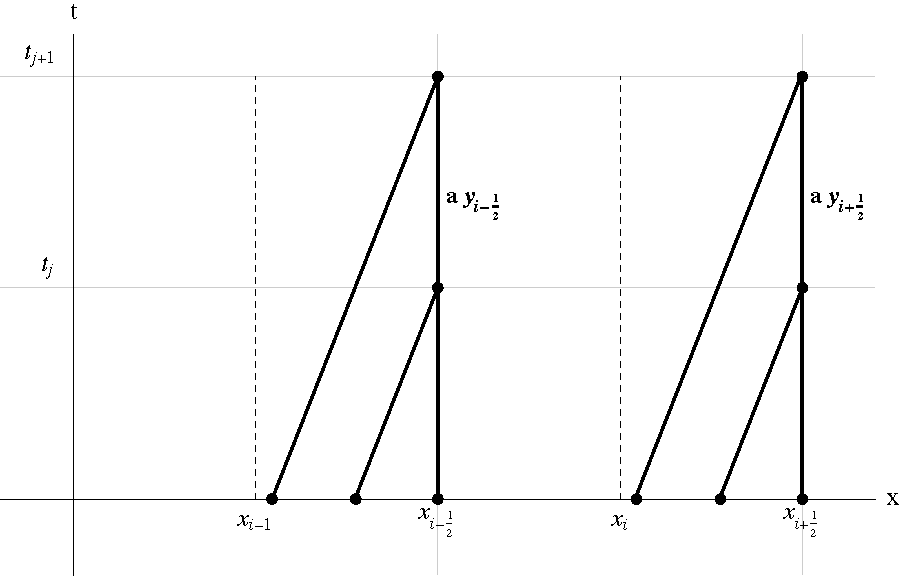
\includegraphics[width=0.95\textwidth]{flow_visual.pdf}
            \caption{Интегрирование потока по пространству, вместо времени}
            \label{fig:flow_visual}
        \end{figure}
    \end{frame}

    \section{Тестирование и сравнение методов}
    \begin{frame}{Анализ точного вычисления граничных и серединных узлов}
        \begin{figure}[h]
            \centering
            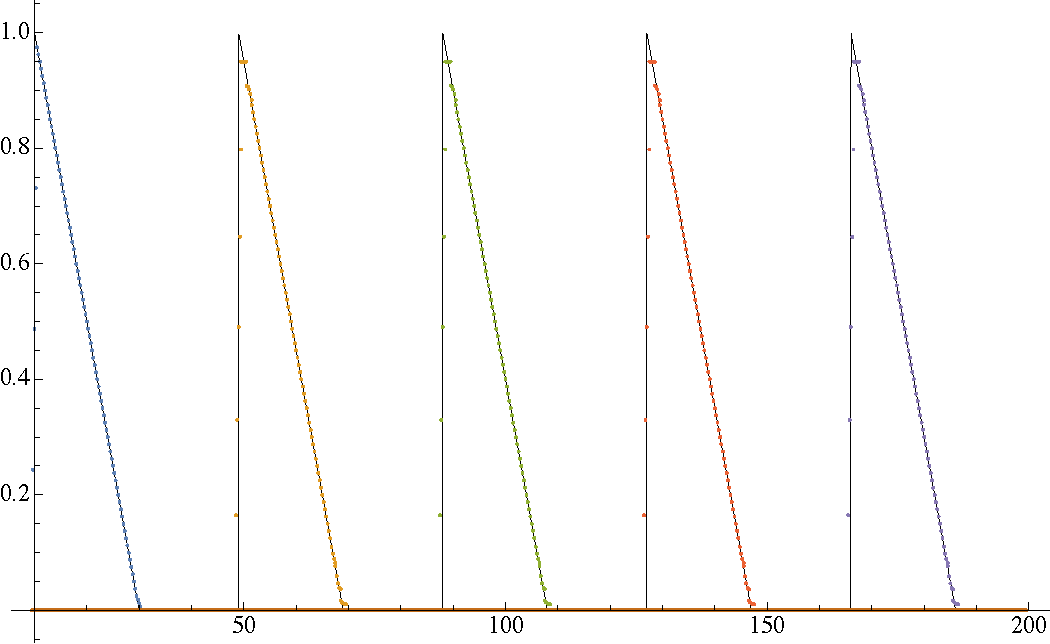
\includegraphics[width=0.72\textwidth]{sigma=1./advectionPPM_rightTriangle.pdf}
            \caption{Правый треугольник для PPM при $ \sigma = 1 $}
            \label{fig:ppm_rightTriangle_1}
        \end{figure}
        \begin{center}
            \begin{tabular}{ |c|c|c|c|c|c| } 
             \hline
              & $ h=1 $ &  $ h=0.5$ &  $ h=0.25 $ &  $ h=0.125 $ &  $ h=0.0625 $ \\ 
             \hline
             $\| \cdot \|_{C}$ & $0.5125$ & $0.506$ & $0.503$ & $0.501$ & $0.5$
             \\
             \hline
             $\| \cdot \|_{L_1}$ & $25.6$ & $6.32$ & $1.57$ & $0.39$ & $0.1$
             \\
             \hline
             $\| \cdot \|_{L_2}$ & $2.89$ & $1.44$ & $0.72$ & $0.36$ & $0.18$ \\
             \hline 
            \end{tabular}
        \end{center}
    \end{frame}

    \begin{frame}{Анализ точного вычисления граничных и серединных узлов}
        \begin{figure}[h]
            \centering
            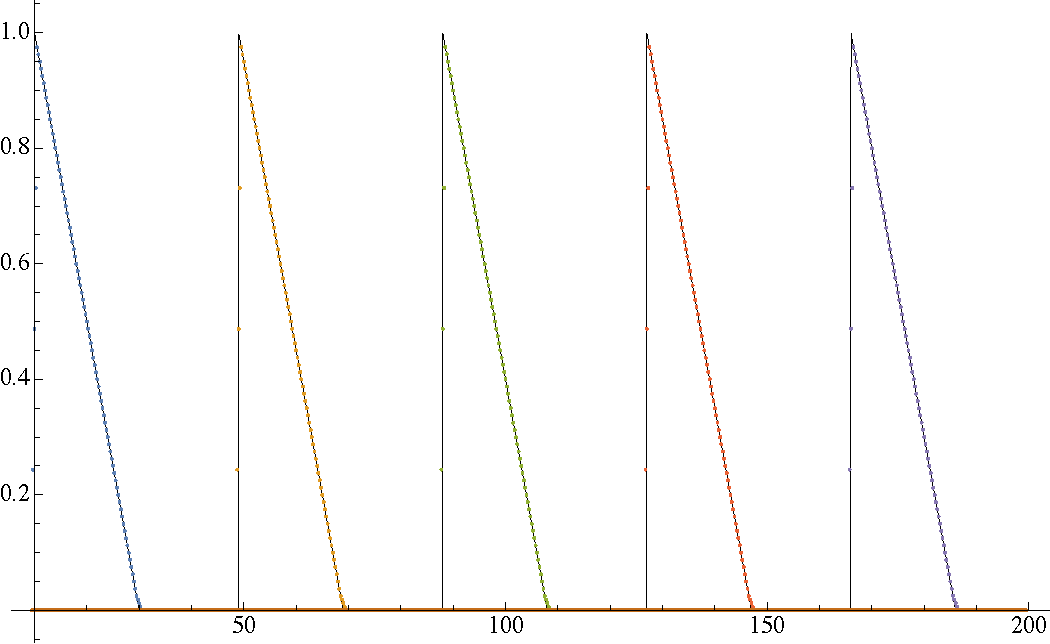
\includegraphics[width=0.72\textwidth]{sigma=1./advectionPPML_rightTriangle.pdf}
            \caption{Правый треугольник для PPML при $ \sigma = 1 $}
            \label{fig:ppml_rightTriangle_1}
        \end{figure}
        \begin{center}
            \begin{tabular}{ |c|c|c|c|c|c| } 
             \hline
            & $ h=1 $ &  $ h=0.5$ &  $ h=0.25 $ &  $ h=0.125 $ &  $ h=0.0625 $ \\ 
             \hline 
             $\| \cdot \|_{C}$ & $0.5125$ & $0.505$ & $0.5029$ & $0.5025$ & $0.5$
             \\
             \hline
             $\| \cdot \|_{L_1}$ & $25.6$ & $6.32$ & $1.57$ & $0.39$ & $0.1$
             \\
             \hline
             $\| \cdot \|_{L_2}$ & $2.86$ & $1.42$ & $0.71$ & $0.305$ & $0.17$
             \\
             \hline
            \end{tabular}
        \end{center}
    \end{frame}

    \begin{frame}{Анализ кусочно-линейного графика при уменьшенном числе Куранта}
        \begin{figure}[h]
            \centering
            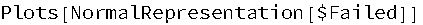
\includegraphics[width=0.66\textwidth]{sigma=0.8/advectionPPM_tooth.pdf}
            \caption{Зуб для PPM при $ \sigma = 0.8 $}
            \label{fig:ppm_tooth_08}
        \end{figure}
        \begin{center}
            \begin{tabular}{ |c|c|c|c|c|c| } 
             \hline
             & $ h=1 $ &  $ h=0.5$ &  $ h=0.25 $ &  $ h=0.125 $ &  $ h=0.0625 $ \\ 
             \hline 
             $\| \cdot \|_{C}$ & $0.716$ & $0.7099$ & $0.7067$ & $0.7023$ & $0.7$
             \\
             \hline
             $\| \cdot \|_{L_1}$ & $41.15$ & $10.14$ & $2.518$ & $0.62$ & $0.3$
             \\
             \hline
             $\| \cdot \|_{L_2}$ & $0.8$ & $0.39$ & $0.195$ & $0.097$ & $0.04$
             \\
             \hline
            \end{tabular}
        \end{center}
    \end{frame}

    \begin{frame}{Анализ кусочно-линейного графика при уменьшенном числе Куранта}
        \begin{figure}[h]
            \centering
            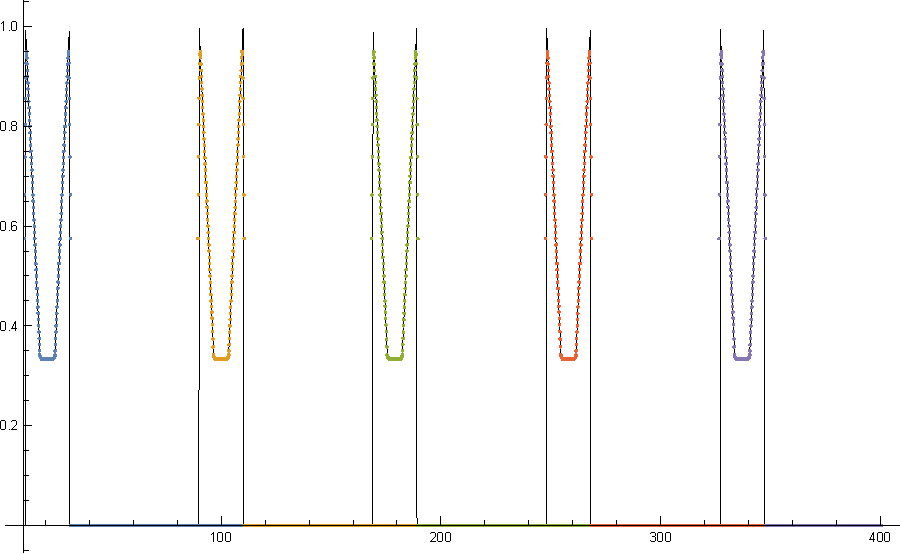
\includegraphics[width=0.66\textwidth]{sigma=0.8/advectionPPML_tooth.pdf}
            \caption{Зуб для PPML при $ \sigma = 0.8 $}
            \label{fig:ppml_tooth_08}
        \end{figure}
        \begin{center}
            \begin{tabular}{ |c|c|c|c|c|c| } 
             \hline
             & $ h=1 $ &  $ h=0.5$ &  $ h=0.25 $ &  $ h=0.125 $ &  $ h=0.0625 $ 
             \\ 
             \hline
             $\| \cdot \|_{C}$ & $0.58$ & $0.56$ & $0.557$ & $0.554$ & $0.55$ 
             \\
             \hline
             $\| \cdot \|_{L_1}$ & $39.85$ & $9.9$ & $2.2$ & $0.56$ & $0.27$
             \\
             \hline
             $\| \cdot \|_{L_2}$ & $0.7$ & $0.34$ & $0.187$ & $0.08$ & $0.03$ 
             \\
             \hline
            \end{tabular}
        \end{center}
    \end{frame}

    \begin{frame}{Анализ методов на гладком графике}
        \begin{figure}[h]
            \centering
            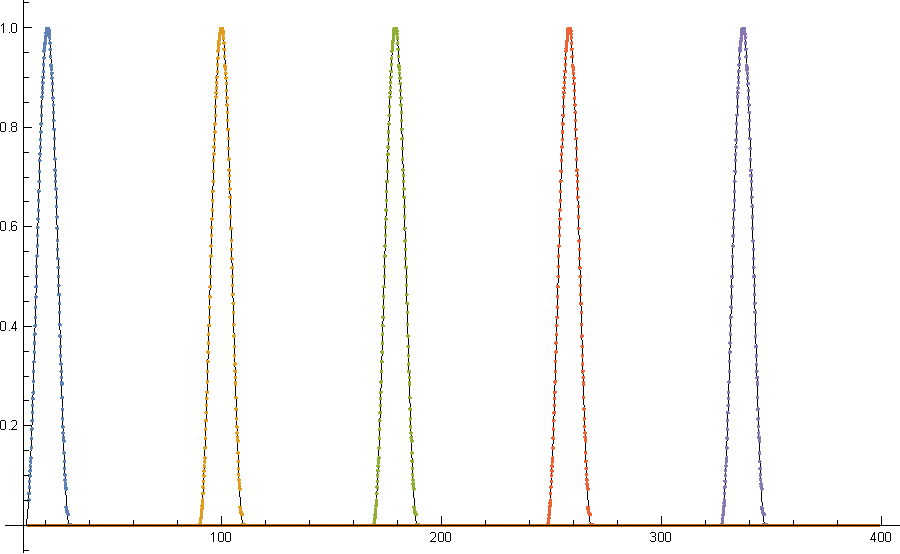
\includegraphics[width=0.66\textwidth]{sigma=0.5/advectionPPM_cos.pdf}
            \caption{Косинус для PPM при $ \sigma = 0.5 $}
            \label{fig:ppm_cos_05}
        \end{figure}
        \begin{center}
            \begin{tabular}{ |c|c|c|c|c|c| } 
             \hline
             & $ h=1 $ &  $ h=0.5$ &  $ h=0.25 $ &  $ h=0.125 $ &  $ h=0.0625 $ \\ 
             \hline
             $\| \cdot \|_{C}$ & $0.244$ & $0.1117$ & $0.044$ & $0.019$ & $1e{-05}$
             \\
             \hline
             $\| \cdot \|_{L_1}$ & $2.59$ & $0.327$ & $0.04$ & $0.005$ & $2e{-05}$
             \\
             \hline
             $\| \cdot \|_{L_2}$ & $0.99$ & $0.18$ & $0.003$ & $0.00055$ & $2e{-05}$ 
             \\
             \hline
            \end{tabular}
        \end{center}
    \end{frame}

    \begin{frame}{Анализ методов на гладком графике}
        \begin{figure}[h]
            \centering
            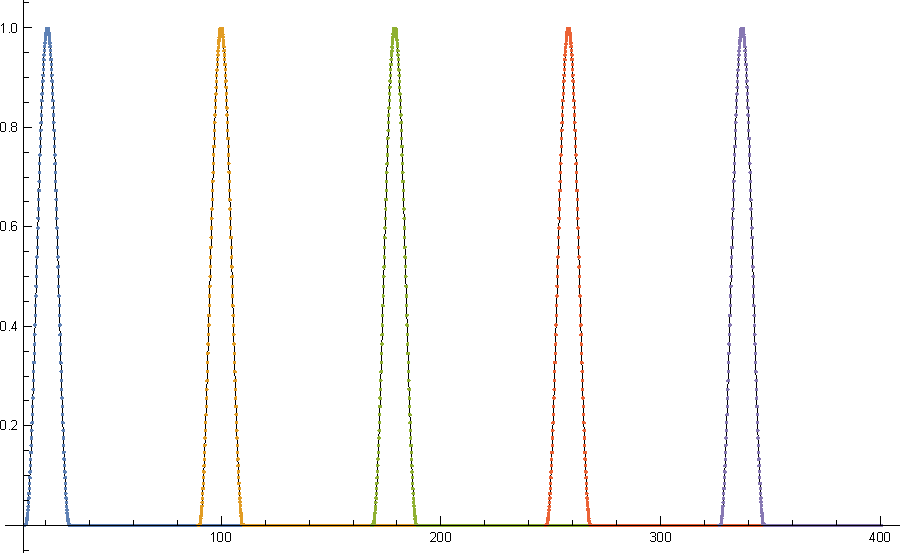
\includegraphics[width=0.66\textwidth]{sigma=0.5/advectionPPML_cos.pdf}
            \caption{Косинус для PPML при $ \sigma = 0.5 $}
            \label{fig:ppml_cos_05}
        \end{figure}
        \begin{center}
            \begin{tabular}{ |c|c|c|c|c|c| } 
             \hline
             & $ h=1 $ &  $ h=0.5$ &  $ h=0.25 $ &  $ h=0.125 $ &  $ h=0.0625 $ \\ 
             \hline
             $\| \cdot \|_{C}$ & $0.048$ & $0.015$ & $0.005$ & $0.0016$ & $1e{-06}$
             \\
             \hline
             $\| \cdot \|_{L_1}$ & $2.55$ & $0.32$ & $0.0398$ & $0.0049$ & $2e{-06}$
             \\
             \hline
             $\| \cdot \|_{L_2}$ & $0.99$ & $0.18$ & $0.003$ & $0.00055$ & $2e{-06}$ 
             \\
             \hline
            \end{tabular}
        \end{center}
    \end{frame}

    \begin{frame}
        \frametitle{Список использованных источников}
        \begin{thebibliography}{9}
  
            \bibitem{Corella} Corella P., Woodward P. The piecewise parabolic method for gas-dynamical simulations // J. Comput. Phys. $1984$. V.$54$. P. $174-201$.
      
            \bibitem{Article} М.\,В.\,Попов, С.\,Д.\,Устюгов. Кусочно-параболический метод на локальном шаблоне для задач газовой динамики, Ж. вычисл. матем. и матем. физ., $2007$, том $47$, номер $12$, $2055-2075$, c. $2056-2060$.
      
            \bibitem{Galanin} Галанин М.П. Методы численного анализа математических моделей/М.П. Галанин, Е.Б. Савенков.–М. : Изд-во МГТУ им. Н.Э. Баумана, 2010.–591, [1] с.: ил. (Математическое моделирование в технике и технологии)
    
            \bibitem{Samarsky} А.\,А.\,Самарский, Ю.\,П.\,Попов. Разностные методы решения задач газовой динамики: Учеб. пособие: Для вузов -- $3$-е изд., доп. -- M.: Наука. Гл. ред. физ. мат. лит., $1992$. -- $424$ с.
    
            \bibitem{Kulikovsky} А.\,Г.\,Куливокский, Н.\,В.\,Погорелов, А.\,Ю.\,Семенов. Математические вопросы численного решения гиперболических систем уравнений. -- М.: ФИЗМАТЛИТ, $2001$. -- $608$ с.
      
        \end{thebibliography}
    \end{frame}

\end{document}